\chapter{Marco Teórico}
\newpage
\section{Power TAC(Trading Agent Competition).}
Es una competencia de simulación modelando un sofisticado mercado energético, donde los competidores broker o agentes deben de obtener ganancias a partir de los elementos que integran a Power TAC. En la figura \ref{entorno} muestra los principales componentes que integra el entorno de simulación de PowerTAC.

\begin{figure}[!h]
    \centering
    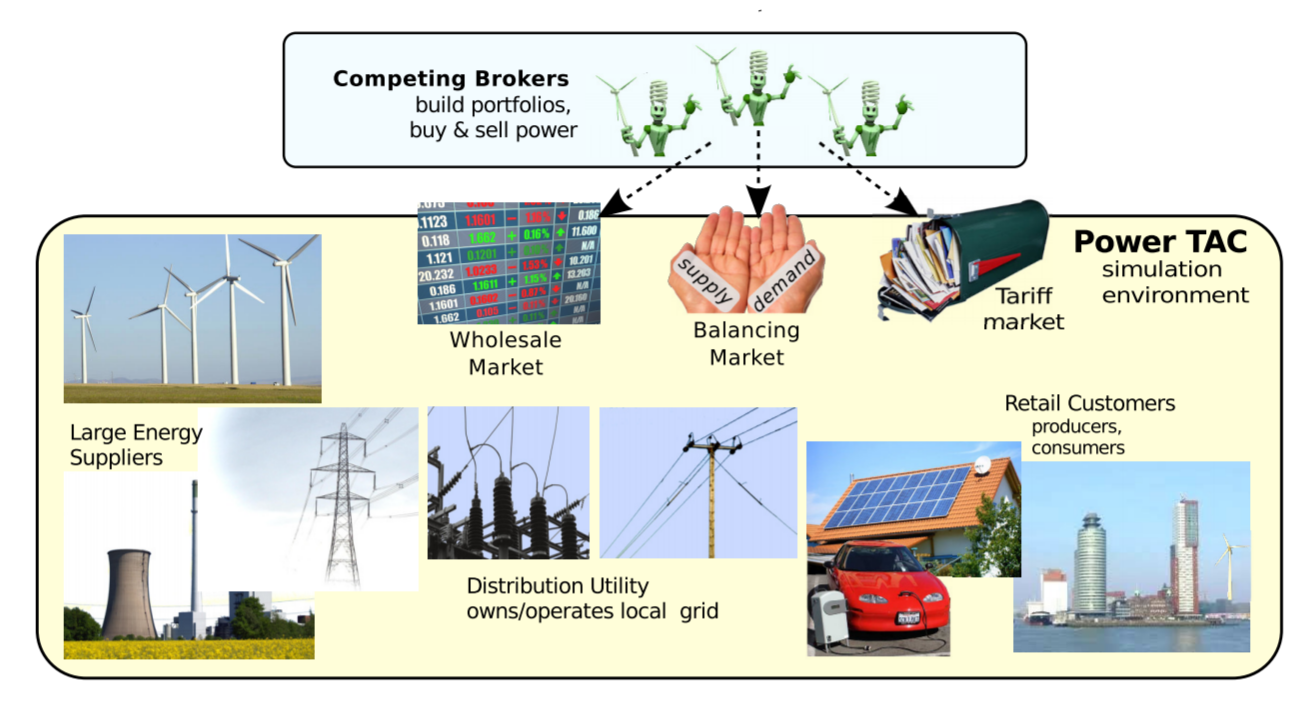
\includegraphics[width=10cm]{img/entorno.png}
    \caption{Elementos del entorno de simulación de Power TAC.}
    \label{entorno}
\end{figure}

A continuación se describen cada uno de los elementos:\\

\textbf{Customer Market.}\\

También es llamado Mercado de Tarifas, por este medio los agente adquiere energía de los productores locales y la vende a sus consumidores. El agente ofrecen contratos o tarifas especificando el precio y otros términos, mientras que los clientes tomas la decisión de aceptarlos o ignorar. La construcción de una tarifa te permite especificar los siguiente términos: especificar periodo de pagos, tiempo de uso, bonos o pagos por suscripción, mínima duración de contrato, pagos de penalización de retiro antes de cumplir con la mínima duración, precisión por consumo y producción, etc. En la sección \ref{tariff} encontrara mas información de la estructura de una tarifa\\

\textbf{Wholesale Market.}\\

Mercado al por mayor permite a los broker comprar y vender energía entre 1 y 24 horas en el  futuro, por este razón también es conocido como mercado del día siguiente. El broker y otros participantes proporcionan energía al por mayor a granel y liquidez al mercado, simulando la demanda de un mercado regional que es sustancialmente mayor que la demanda representada por el escenario de simulación de energía TAC.\\

\textbf{Distribution Utility.}\\

El Distribuidor de Utilidades (DU) modela el monopolio regulador y mantiene la infraestructura de distribución de energía. Dentro del contexto de Power TAC participa en los siguientes escenarios:

\begin{enumerate}
    \item Encargado de distribuir la energía de la red a los clientes. Implicado pagos por el uso de la distribución de la energía hacia los clientes.
    \item Permite importar y exportar energía desde el Mercado al por Mayor.
    \item Actúa como broker de última instancia, ofreciendo sencillas tarifas clientes de consumo y de producción de energía.
\end{enumerate}

\textbf{Balancing Market.}\\

El mercado de balance es el encargo de mantener el equilibrio entre la oferta y la demanda en la distribución en la red. Ll Mercado de Balance mantiene un sistema de incentivo para los broker por mantener el equilibrio entre la oferta y la demanda de su portafolio de clientes en cada intervalo de tiempo, logrando reducir el costo de las penalizaciones de desbalance realizadas por el DU.

\textbf{Accounting.}\\

Para garantizar la coherencia y la imparcialidad, el simulador de Power TAC mantiene un registro de las cuentas de los agentes, las suscripciones de los clientes y las posiciones en el mercado al por mayor. Ademas mantiene un registro las siguientes transacciones:

\begin{itemize}
    \item Suscripción y retiro de clientes por tarifa.
    \item Consumo y producción de energía por cliente.
    \item Pagos por publicación de tarifas.
    \item Pagos por distribución.
    \item Pagos del Mercado al por mayor.
    \item Pagos del Mercado de Balance.    
\end{itemize}

Cada agente tiene una cuenta en efectivo en el banco central, e inicia el juego con un saldo de cero en la cuenta. Los créditos y débitos de las distintas transacciones se agregan a la cuenta durante cada timeslot.\\

\textbf{Weather reports.}\\

El pronostico meteorológico y las condiciones meteorológicas actual se envían a los broker en cada intervalo de tiempo. Algunos modelos de clientes utilizarán esta información para influir en el consumo de energía y en la producción. Los informes meteorológicos y las predicciones se extraerán de los datos meteorológicos y de pronósticos del mundo real para. La ubicación específica y el intervalo de fechas para el conjunto de datos meteorológicos son información privilegiada, no revelada a los agentes, sin embargo se dan la latitud y época del año.\\

\textbf{Tiempo de simulación.}\\

El tiempo de simulación en Power TAC se divide por time slot cada uno con una duración de una hora en tiempo de simulación, cada times slot tienen un a duración de 5 segundos en tiempo real, las rondas de simulación consisten en 60 días de simulación equivalente a 1440 timeslot o aproximadamente a 2 horas en tiempo real.\\

\section{Broker.}

El broker es el responsable de ser el intermediario entre las negociaciones en el Mercado de Tarifas, Mercado al por Mayor y el Mercado de Balance, con el objetivo de lograr ganancias a partir de la compra y venta de energía. Durante un times slot el agente puede realizar algunas de las actividades de la figura \ref{activity}.

\begin{figure}[!h]
    \centering
    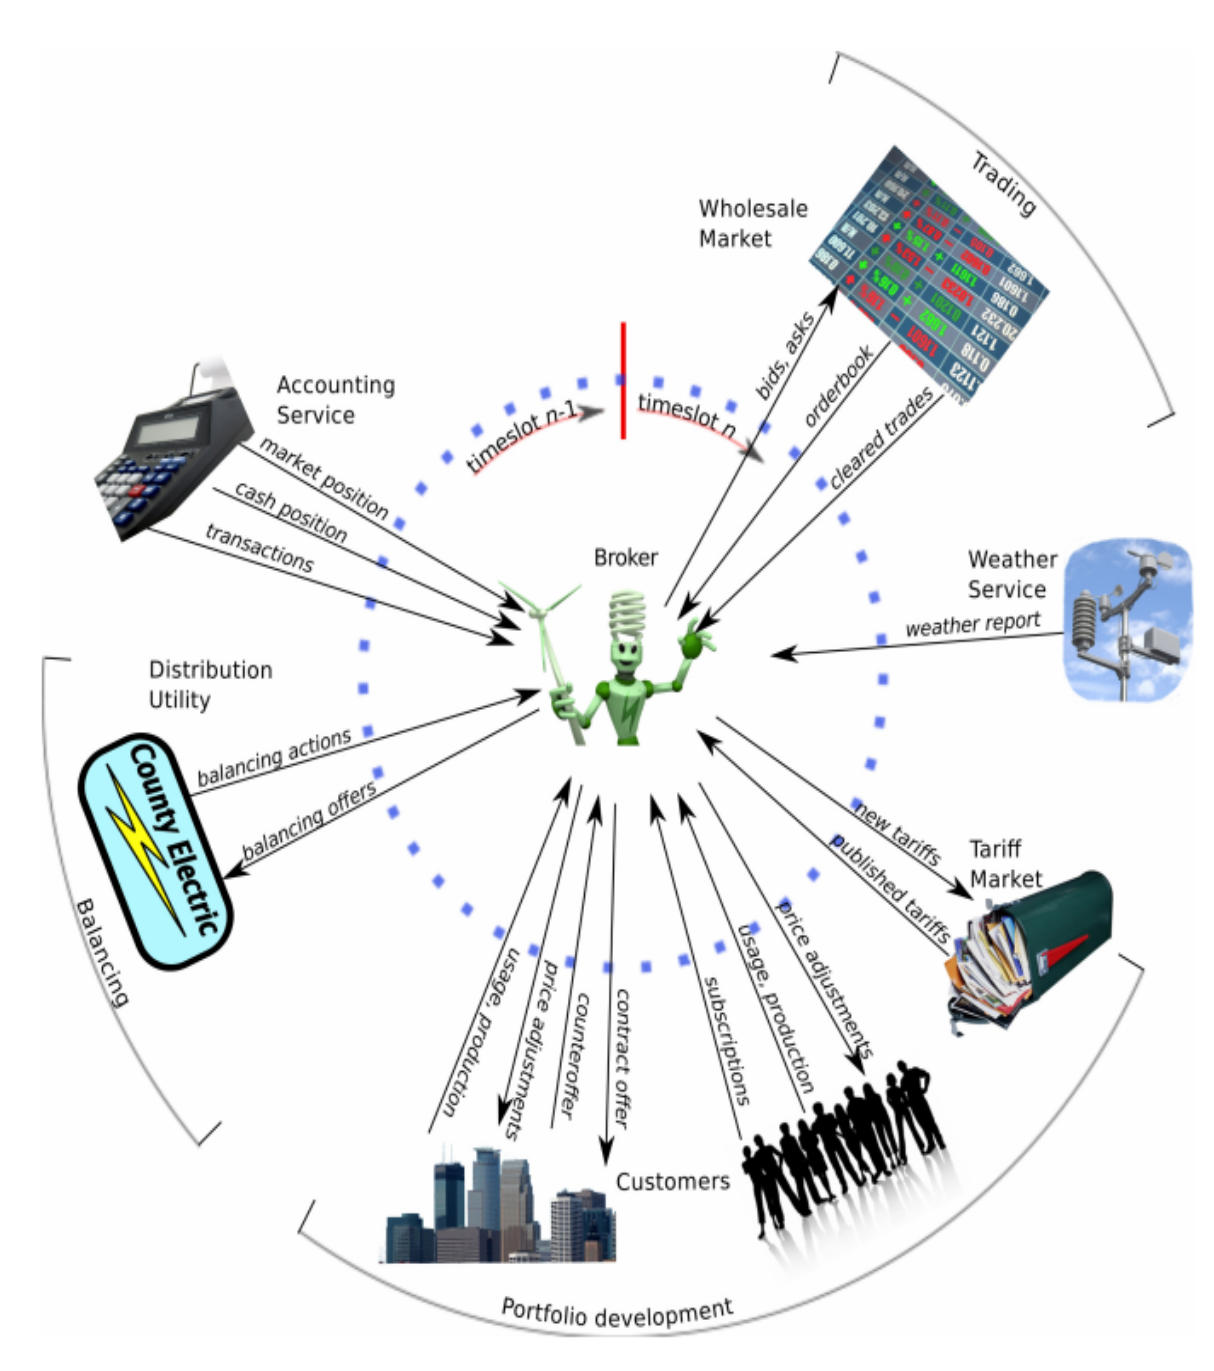
\includegraphics[width=8cm]{img/process.png}
    \caption{Actividades realizadas por el broker en un time slot.}
    \label{activity}
\end{figure}

\begin{description}
    \item [Oferta de tarifas (Mercado de Tarifas):] crea y publica nuevas tarifas.
    \item [Modificación de tarifas (Mercado de Tarifas):]  cambia las condiciones de una tarifa reemplazandola por una nueva.
    \item [Ajuste de precios (Clientes):] ajustar los precios de las tarifas ya existentes.
    \item [Recortar la demanda (Clientes):] para los clientes que han suscrito a las tarifas que permiten capacidades controlables, los broker pueden ejercer restricciones para gestionar la demanda.
    \item [Publicar ordenen de balance (Mercado de Balance):] proporcionar al mercado de balance clientes con capacidades controlables para contribuir al desbalance de la red.
    \item [Enviar solicitudes y ofertas (Mercado al por Mayor):]  crear solicitudes y ofertas para vender y adquirir energía para los futuros time slot.
\end{description}

\section{Tarifas.}
\label{tariff}
Las tarifas son la relación existente entre un broker y sus clientes, es decir es un contrato que especifica una serie de condiciones asociadas al precio, minima duración de contrato, bonos y pagos por suscripción, etc. Los broker son los encargados de crear tarifas específicas a partir de un estructura definida  en la figura \ref{tariff}. La estructura de una tarifa puede variar dependiendo al PowerType que esté sujeta a ella.

\begin{figure}[h!]
    \centering
    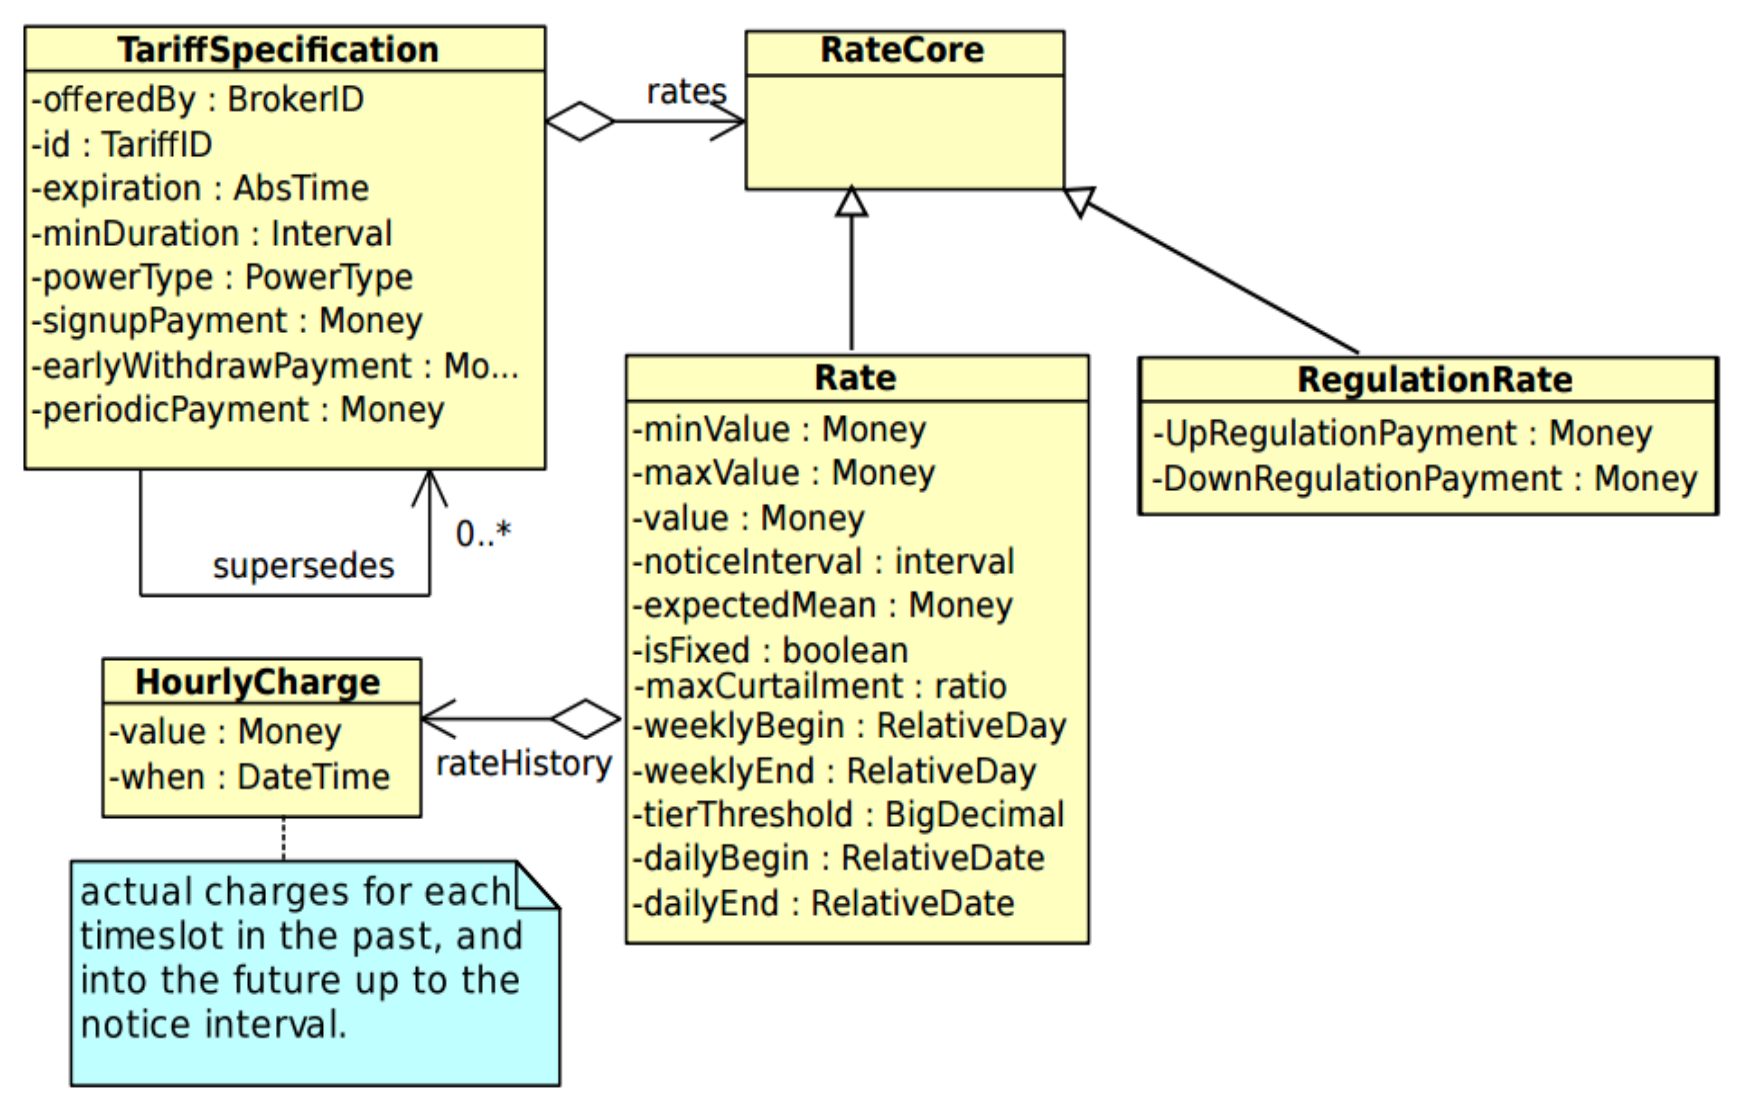
\includegraphics[width=13cm]{img/tariffstructe.png}
    \caption{Clases asociadas a la estructura de una tarifa.}
    \label{tariff}
\end{figure}

Muchos de los elementos son representados en una  TariffSpecification donde podemos indicar las condiciones del pago y el PowerType, pero el precio se especifica en la estructura Rate.\\

Muchos de los elementos son representados en TariffSpecification donde podemos indicar las condiciones del pago y el PowerType, pero el precio se especifica en la estructura Rate. La cantidad de dinero y de energía especificado en  TariffSpecification es visto desde el punto de vista de un cliente, es decir se para el dinero si es valor es negativo representa una pago del cliente y el broker, mientras un valor positivo representa un pago desde el broker al cliente. Similar mente una cantidad de energía representado en kWh con un valor positivo representa energia entregada al cliente y un valor negativo es la energía entregada al broker.\\

Cuando el broker publica una tarifa esta debe de pasar por una serie de estados en la figura \ref{state} muestra los estados de un tarifa.  El broker envia una tarifa al mercado de tariff y esta entra en estado de “pending”. La nueva tarifas es publicasd periodicamente a los clientes y a los broker, entrando al estado “Offered”, los clientes se suscribe y la tarifa entra en un estado “active”. Imediatamente el broker es notificado de varios eventos entre ellos, suscricion de clientes,  cancelacion de contrato, entre otras aciones. Los tarifas pueden tener una fecha de vencimiento y no se permiten nuevas suscripciones en este caso entra en un estado de “expired” hasta que esta es revocada o modificado por un broker.

\begin{figure}[h!]
    \centering
    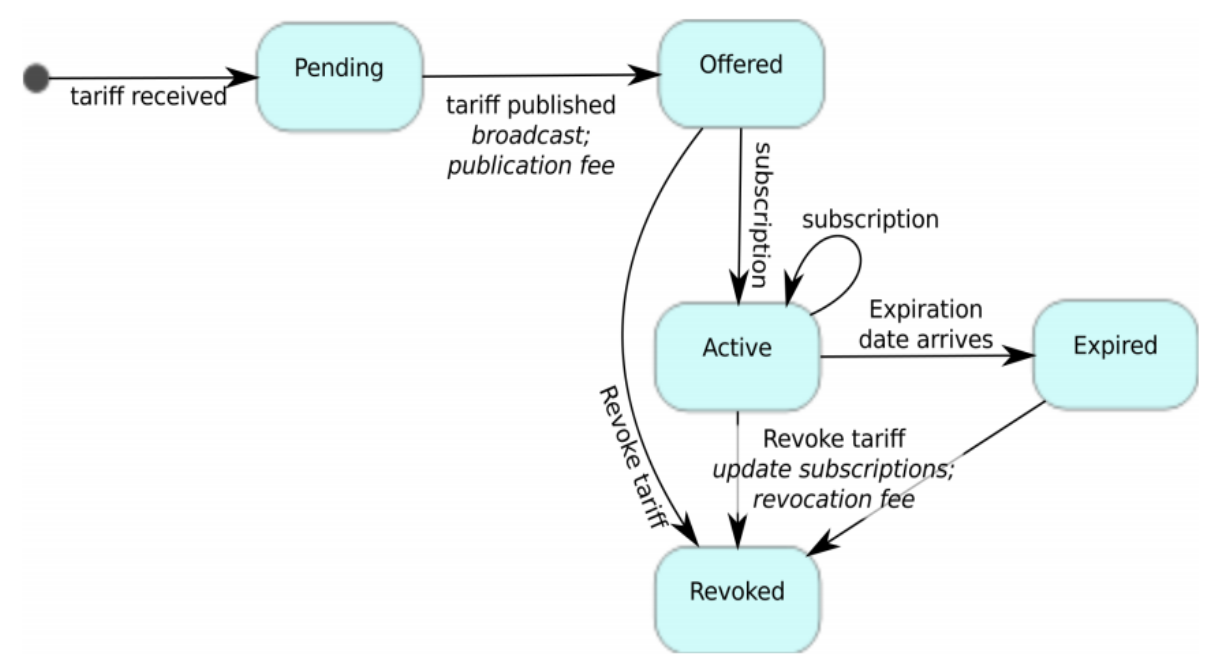
\includegraphics[width=10cm]{img/state.png}
    \caption{Estados de un tarifa.}
    \label{state}
\end{figure}

\section{Customer.}

Power TAC ofrece modelos de clientes que interactúan con los broker mediante el mercado de tarifas. Cada uno de los clientes se caracteriza por un comjunto de información que incluye:

\begin{description}
  \item[Name:] un identificador único.
  \item[Population:] un entero representando el numero de entidades indivisibles (casa, oficinas, vehiculos electricos).
  \item[PowerType:] indica siun cliente es de producion o de consumo, ademas indica si  son controlables o de almacenamiento.
  \item[Controllable capacity:] son indicado por tres atributos: controlableKW  es el total de capacidad en kWh, up-regulation un rango máximo de descarga en kW y down-regulation un rango de máximo en kW de almacenamiento. Si estos tres números están en cero indica que este cliente no tiene capacidades controlables.
  \item[MultiContracting:] es la capacidad del cliente en particionar la población sobre múltiples tarifas.
  \item[CanNegotiate:] este campo indica que el cliente tiene la capacidad de negociar contratos individuales. Este campo por el momento no tiene utilidad para la competencia del 2017.
\end{description}







\section{Procesos de Decisión de Markov.}
Las técnicas Markovianas modelan un problema de decisión secuencial, definido por un conjunto de estados, un conjunto de acciones posibles, un modelo del entorno y una función de recompensas, que sirve como medio de interacción entre el entorno y el agente. Sus dominios se modelan como sistemas estocásticos, sus metas se definen por sus funciones utilidad/coste (recompensa/descuento), donde el problema de planificación se transforma en un problema de optimización. De ahí que su solución sea la política óptima, asignando la mejor acción en cada estado del espacio de estados del problema.\\

Al problema de encontrar una estrategia reactiva de control (o política de acción) en problemas de decisión secuencial, que maximice la recompensa esperada en el tiempo, se le conoce como proceso de decisión de Markov o MDP (por sus siglas en inglés Markov Decision Process). El trabajo de Markov supone que el agente siempre conoce el estado en que se encuentra al momento de iniciar la ejecución de sus acciones y que la probabilidad de transición depende solamente de este estado y no de su historia, es decir cumple con la propiedad de Markov\footnote{La Propiedad de Markov se refiere a la propiedad de ciertos ambientes estocásticos, donde la distribución de la probabilidad del valor futuro de una variable aleatoria depende únicamente de su valor presente, siendo independiente de la historia de dicha variable.}, afectada por un factor de descuento que impacta negativamente a la utilidad

\subsection{Definición Matemática.}
Los MDPs proveen un marco matemático intuitivo para modelar problemas de decisión secuencial en ambientes dinámicos inciertos . Formalmente un MDP es una 4-tupla:
$$M=< S,A,T,R >$$
Donde:\\
$S$ = conjunto de estados $\{s_{1},...,s_{n}\}$.\\
$A$ = conjunto de acciones $\{a_{1},...,a_{n}\}$.\\
$T$ = función de transición de un estado $s$ a $s'$.\\
$R$ = función de recompensa de un estado $s$ a $s'$ mediante una acción.\\

\section{Métodos de Resolución.}
Recordemos que la tarea del agente es encontrar una política que maximice alguna medida de refuerzo. Su optimización conduce a la obtención de un sistema de ecuaciones no lineales debido a que contienen una maximización. Existen varios métodos de resolución de MDPs, basándose en el conocimiento completo del MDP se clasifican de la siguiente forma:

\begin{itemize}
\item Programación dinámica.
\item Programación lineal.
\item Aprendizaje por refuerzo.
\end{itemize}

La primeras dos técnicas se distingue por conocen el MDPs, es decir tienen conocimiento del conjunto de estado, conjunto de acciones, de la función de transición y la función de recomienza. En cambio la tercera no tiene acceso a esta información, por lo que requiere explorar para aprender estados probables, resultando por ello más compleja que las dos primeras y con la posibilidad de que no se cumpla con la propiedad de Markov.

\subsection{Programación Dinámica.}
La programación dinámica se basa en el principio de optimalidad de Bellman\footnote{Principio de Optimalidad de Bellman: "dada una secuencia óptima de decisiones, toda subsecuencia de ella es, a su vez, óptima"}, lo que tratan de conseguir los algoritmos de programación dinámica es el mantenimiento de las funciones de valor $V (s)$ o $Q(s, a)$ de forma que una vez obtenidos los valores óptimos de estas funciones se pueda derivar de ellas la política óptimas.\\

Los distintos enfoques de programación dinámica explícitamente almacenan funciones de valor del espacio de estados e iterativamente actualizan los valores para cada estado, hasta que el cambio de la función de valor es menor o igual al umbral previamente establecido. Entonces se dice que la función de valor converge a su valor óptimo, con su correspondiente acción o política óptima. Por lo que la programación dinámica ofrece un enfoque unificado para resolver problemas de control estocástico como lo son los MDPs. Los métodos más populares de programación dinámica son el algoritmo de iteración de valor y el algoritmo de iteración de política.

\subsubsection{Iteración por Valor.}
El algoritmo de iteración de valor aplica actualizaciones sucesivas de la función de valor para cada estado $s \in S$, al ejecutar el Principio de Optimalidad de Bellman, siendo la recompensa inmediata del estado en evaluación su valor inicial. De esta manera se actualiza la utilidad de cada estado a partir de las utilidades de sus estados vecinos inmediatos. Entonces se repite el proceso hasta que alcanza la convergencia. Cabe destacar que si esta actualización se aplica indefinidamente, entonces queda garantizado que se alcanzará un estado de equilibrio. El proceso se detiene cuando la diferencia entre las dos últimas iteraciones es menor que el máximo error permitido. Entonces, la iteración de valor converge finalmente a un único conjunto de soluciones. A continuación se muestra el algoritmo de Iteración por Valor.

\subsubsection{Iteración por Política.}

Una política $\pi$ define el comportamiento de un agente aprendiz en un momento dado. En otras palabras, una política es un mapeo de un conjunto de estados $S$ percibidos del ambiente a un conjunto de acciones $A$ que deben ejecutarse en dichos estados. En algunos casos la política puede ser una función simple o una tabla de entradas, y en otros casos puede ser un proceso complejo de búsqueda. En general, las políticas pueden ser estocásticas.

$$\pi : S \rightarrow A$$\\

Otro algoritmo de programación dinámica es la iteración de política, en este método, la política es repetidamente mejorada al encontrar una acción en cada estado que tenga un valor más alto que el valor de la acción escogida anteriormente para ese estado. La política inicial es aleatoria y el proceso termina cuando ya no es posible realizar más mejoras. Cabe señalar que este proceso garantiza la convergencia a la política óptima.
La dinámica de este algoritmo es la siguiente: toma al MDP, a un valor de descuento, a un parámetro de convergencia y produce políticas óptimas de horizonte finito sucesivas, terminando cuando el máximo cambio entre la función del valor actual y la del valor previo es menor que el margen de error dado. De esta manera logra la convergencia y se detiene. A continuación se muestra el algoritmo de Iteración por Políticas:

\subsection{Programación Lineal.}

Esta técnica resuelve un problema indeterminado formulado a través de ecuaciones lineales, para ello cuenta con el método Simplex. Este método fue desarrollado por G. B. Dantzig en 1947 y consiste en la optimización de la función objetivo al considerar las restricciones habidas. Estas restricciones son desigualdades que acotan a la región que contiene a todos los valores factibles para dichas expresiones matemáticas. Con este método, la iteración toma el valor de un vértice e investiga si es su máximo valor, de no ser así repite el proceso en forma iterativa hasta encontrarlo.

\section{Aprendizaje por Refuerzo.}
El aprendizaje por refuerzo consiste en aprender qué acciones realizar, dado el estado actual del ambiente, con el objetivo de maximizar una se\~{n}al de recompensa numérica, lo cual requiere de un mapeo de situaciones a acciones. El sistema que aprende debe descubrir por sí solo cuales son las acciones que le dan a ganar más. En los casos más interesantes y difíciles, las acciones pueden afectar no sólo la recompensa inmediata sino también la siguiente situación,y de esta forma afectar las siguientes recompensas. Estas dos características, prueba y error, y recompensas retrasadas, son las dos características más sobre salientes del aprendizaje por refuerzo.\\

En caso de que no se cuente con la función de transición de estados ni con la función recompensa del problema, el planificador deberá explorar su entorno para aprender qué hacer y cómo relacionar situaciones (estados) con acciones, de manera que la recompensa sea maximizada. El aprendizaje por refuerzo está basado en la interacción constante de un agente con su entorno incierto, por lo que existe un fuerte compromiso exploración-explotación: la información de entrada es la retroalimentación que obtiene del mundo exterior como respuesta a sus acciones. De ahí este aprendizaje sea cercano a la teoría óptima de control y la aproximación estadística.\\

Mediante la función de aprendizaje por refuerzo, el agente determina cuáles estados son más provechosos a corto plazo. A diferencia de la técnica anterior, la función evaluación es hecha a largo plazo, considerando a los estados a los que puede conducir una acción. De esta manera, sus programas de cómputo buscan ir aprendiendo por sí solos conforme van adquiriendo experiencia, tal y como sucede con el ser humano. En consecuencia, los métodos de solución que utilizan aprendizaje por refuerzo son inductivos. La idea central es hacer uso de la estructura inherente de los MDPs, cuyos estados y acciones pueden ser abstraídos en subpolíticas. Una vez que explora y obtiene información de su entorno, este método se torna informado, pudiendo ser resuelto mediante los métodos de programación dinámica o programación lineal antes descritos.\\

A continuación se muestran los algoritmos que se emplean para aprender la dinámica del entorno:
\begin{itemize}
\item Algoritmos de Equivalencia de Certeza.
\item Dyna-Q.
\item Queue-Dyna.
\item Métodos de Monte Carlo.
\item Métodos de diferencia temporal.
\end{itemize}

Desde el punto de vista del uso que se haga de la política que se está aprendiendo los métodos de este enfoque se pueden clasificar adicionalmente en:
\begin{itemize}
\item Métodos on-policy.
\item Métodos off-policy.
\end{itemize}
%\begin{table}[h!]
% \begin{center}
% \begin{tabular}{|l|l|l|l|l|} \hline
% Minimun\\
% Duration
% &
% PowerType
% &
% Signup Paymen
% &
% Early Withdraw Payment
% &
% Periodic Payment\\
% \hline
% \end{tabular}
% \caption {Clasificación de acuerdo al numero de atributos.}
% \label{clasA}
% \end{center}
% \end{table}